%%%%%%%%%%%%%%%%%%%%%%%%%%%%%%%%%%%%%%%%%%%%%%%%%%%
%
%  New template code for TAMU Theses and Dissertations starting Fall 2012.  
%  For more info about this template or the 
%  TAMU LaTeX User's Group, see http://www.howdy.me/.
%
%  Author: Wendy Lynn Turner 
%	 Version 1.0 
%  Last updated 8/5/2012
%
%%%%%%%%%%%%%%%%%%%%%%%%%%%%%%%%%%%%%%%%%%%%%%%%%%%
%%%%%%%%%%%%%%%%%%%%%%%%%%%%%%%%%%%%%%%%%%%%%%%%%%%%%%%%%%%%%%%%%%%%%%
%%                           SECTION III
%%%%%%%%%%%%%%%%%%%%%%%%%%%%%%%%%%%%%%%%%%%%%%%%%%%%%%%%%%%%%%%%%%%%%



\chapter{\uppercase{Fuel Depletion Problem}}
\label{sec:chapter5_depletion}

We now consider a fuel depletion problem to illustrate that self-lumping DFEM schemes remain accurate for more complex physics than simply a purely absorbing medium.
The depletion method we use [time stepping scheme, time step size, etc.] is chosen for its simplicity, not for its fidelity relative to state-of-the art depletion methodologies.  
Our goal is to assess the accuracy of {\emph spatial discretization} methods for problems with spatially varying cross sections, not to propose a new depletion method.  
However, we stress that self-lumping methods can be implemented with any time depletion method or time stepping scheme since implementation of self-lumping  only requires changes pertaining to the spatial discretization. 

\section{Problem Physical Description}

We will consider a 1-D slab fuel depletion problem.
The dimensions and layout of the fuel and moderator layers lattice is shown in \fig{fig:lattice}.  
\begin{figure}[!htp]
\begin{center}
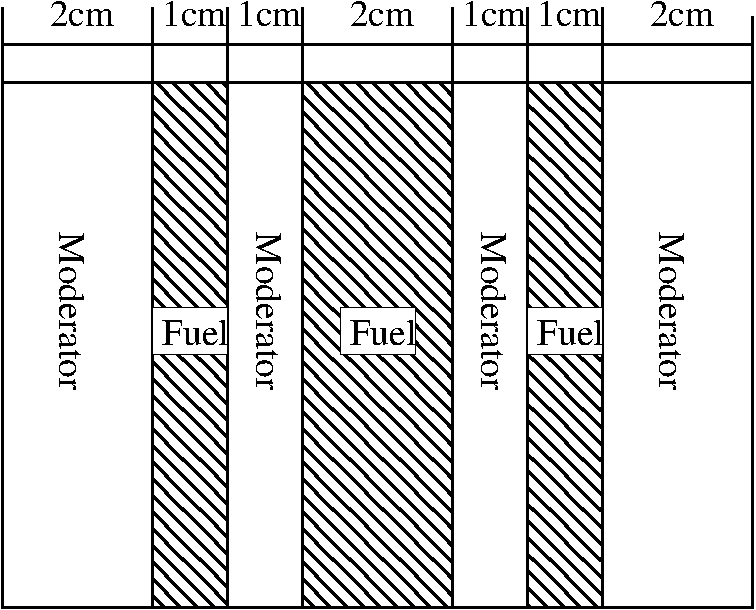
\includegraphics[width=8cm]{chapter5_depletion/article_grid.pdf}
\end{center}
\caption{Depletion problem fuel/moderator lattice.}
\label{fig:lattice}
\end{figure}

Initially, each fuel region is a homogeneous mixture containing only fissile $^{235}U$ and fertile $^{238}U$ nuclei, with compositions given in \tbl{tbl:fuel_atom_density}.
\begin{table}[!htp]
\centering
\caption{Fuel atom density data.}
\begin{tabular}{|c|c|}
\hline
Fuel Density $[g/cm^3]$  & 10.97 \\
\hline
Atom Fraction $^{235}\text{U}$	& 0.05 \\
\hline
Atom Fraction $^{238}\text{U}$ & 0.95 \\
\hline
Fuel Molecular Weight $[amu]$ & 270.03\\
\hline
\end{tabular}
\label{tbl:fuel_atom_density}
\end{table}
%
As fuel depletion progresses, the isotopic composition of fuel changes.
The moderator is light water and its composition, given in \tbl{tbl:water_atom_density}, does not change with irradiation.
\begin{table}[!htp]
\centering
\caption{Water atom density data.}
\begin{tabular}{|c|c|}
\hline
Water Density $[g/cm^3]$  & 1 \\
\hline
Atom Fraction $^1\text{H}$	& $\frac{2}{3}$ \\
\hline
Atom Fraction $^{16}\text{O}$ & $\frac{1}{3}$ \\
\hline
Water Molecular Weight $[amu]$ & 18.02\\
\hline
\end{tabular}
\label{tbl:water_atom_density}
\end{table}
We track five nuclide types in the fuel during the fuel depletion problem: fissile, fertile, parasitic absorber fission product, scattering fission product, and inert, whose spatial nuclide densities, $[atom/cm^{3}]$, are respectively denoted as $N_{FS}$, $N_{FT}$, $N_{FP-A}$, $N_{FP-S}$, and $N_I$.

We use a two-energy-group approximation with the standard numbering convention- the lower the group number, the faster the neutron.  
All neutrons are born fast, there is no thermal upscattering, and we assume all scattering and fission is isotropic in angle.
We also assume that if neutron absorption leads to isotopic transmutation, the transmutation occurs at the time of absorption, there are no radioactive decay chains.
All possible transmutation paths are shown in \fig{fig:transmutation}.
\begin{figure}[!htp]
\begin{center}
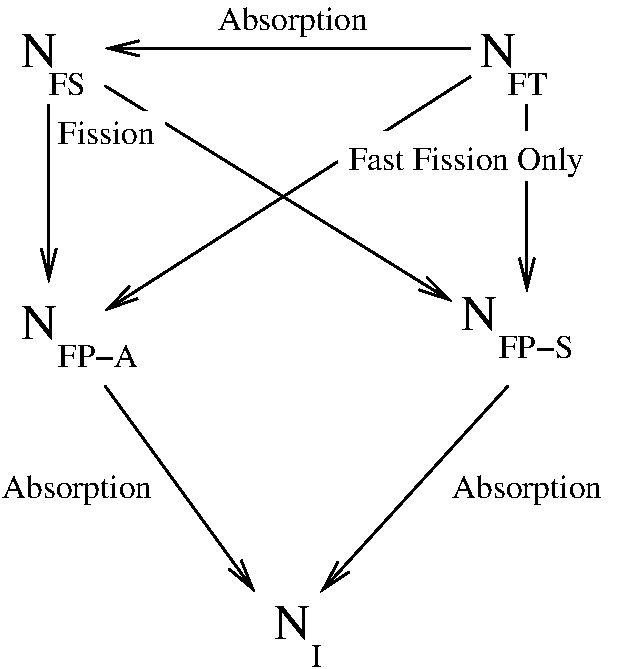
\includegraphics[width=10cm]{chapter5_depletion/article_transmutation.pdf}
\end{center}
\caption{Depletion problem possible transmutation paths and mechanisms.}
\label{fig:transmutation}
\end{figure}

Under these assumptions, and given the transmutation paths given in \fig{fig:transmutation}, the fully analytic, nonlinear depletion equations are:
\begin{subequations}
\label{eq:analytic_depletion}
\benum
\mu \frac{\partial  \psi_1}{\partial  x} + \Sigma_{t,1} \psi_1 = \frac{\Sigma_{s,1\to 1}}{4\pi}\phi_1 + \frac{1}{k}\left( \frac{\nu\Sigma_{f,1}}{4\pi}\phi_1 + \frac{\nu\Sigma_{f,2}}{4\pi}\phi_2 \right)
\eenum
\benum
\mu \frac{\partial  \psi_2}{\partial  x} + \Sigma_{t,2} \psi_2 = \frac{\Sigma_{s,2\to 2}}{4\pi}\phi_2 +
\frac{\Sigma_{s,1\to 2}}{4\pi}\phi_1 
\eenum
\begin{multline}
\frac{\partial N_{FS}}{\partial t} = -N_{FS}\left[(1-\gamma_{FS,1})\sigma_{a,FS,1}\phi_1 + (1-\gamma_{FS,2})\sigma_{a,FS,2}\phi_2 \right] \\  + N_{FT}[\gamma_{FT,1}\sigma_{a,FT,1} \phi_1 + \gamma_{FT,2}\sigma_{a,FT,2}\phi_2  ] 
\end{multline}
%
%
\benum
\frac{\partial N_{FT}}{\partial t} = -N_{FT}[\sigma_{a,FT,1}\phi_1 + \sigma_{a,FT,2}\phi_2] 
\eenum
%
%
\begin{multline}
\frac{\partial N_{FP-S}}{\partial t} = N_{FS} \left[ (1-p_{FS,1})y_{FS,1}\sigma_{a,FS,1}\phi_1 +  (1-p_{FS,2})y_{FS,2}\sigma_{a,FS,2}\phi_2 \right] \\
+ N_{FT}\left[ (1-p_{FT,1})y_{FT}\sigma_{a,FT,1}\phi_1 \right] 
- N_{FS}\left[\sigma_{a,FP-S,1}\phi_1 + \sigma_{a,FP-S,2}\phi_2  \right]
\end{multline}
%
%
%N_{fs}\int_0^{\inFTy}{\left[dE~(1-p_{fs})y_{fs}\sigma_{a,fs} \phi\right]} + 
%N_{FT}\int_0^{\inFTy}{\left[dE~ (1-p_{FT}) y_{FT} \sigma_{a,FT} \phi \right]} \\
%
%

\begin{multline}
\frac{\partial N_{FP-A}}{\partial t} = N_{FS}\left[ p_{FS,1} y_{FS,1} \sigma_{a,FS,1}\phi_1 + p_{FS,2} y_{FS,2} \sigma_{a,FS,2}\phi_2  \right] \\
+ N_{FT} p_{FT,1} y_{FT,1}\sigma_{a,FT,1}\phi_1  \\
- N_{FP-A}\left[ (1-\xi_{FP-A,1})\sigma_{a,FP-A,1}\phi_1 + (1-\xi_{FP-A,2})\sigma_{a,FP-A,2}\phi_2  \right] 
\end{multline}
%N_{fs}\int_0^{\inFTy}{\left[dE~p_{fs} y_{fs} \sigma_{a,fs} \phi \right]} + 
%N_{FT} \int_0^{\inFTy}{\left[dE~p_{FT} y_FT\sigma_{a,FT} \phi\right]} - 
%N_{FP-A}\int_0^{\inFTy}{\left[ dE~ (1-\xi_{FP-A})\sigma_{a,FP-A}  \phi \right]}   \\
%
%
\begin{multline}
\frac{\partial N_I}{\partial t} = 
%N_{FT}\left( (1-\gamma_{FT,1})(1-y_{FT,1})\sigma_{a,FT,1} \phi_1 + (1-\gamma_{FT,2})(1-y_{FT,2})\sigma_{a,FT,2}\phi_2  \right) \\
%+ N_{fs}\left( (1-\gamma_{fs,1})(1-y_{fs,1})\sigma_{a,fs,1}\phi_1 + (1-\gamma_{fs,2})(1-y_{fs,2})\sigma_{a,fs,2}\phi_2 \right) \\
N_{FP-A} \left[  \xi_{FP-A,1}\sigma_{a,FP-A,1}\phi_1 + \xi_{FP-A,2}\sigma_{a,FP-A,2}\phi_2 \right] \\
+ N_{FP-S}\left[ \sigma_{a,FP-S,1}\phi_1 + \sigma_{a,FP-S,2}\phi_2  \right]\pep
\end{multline}
\end{subequations}

In Eq. (\ref{eq:analytic_depletion}a) and Eq. (\ref{eq:analytic_depletion}b) 
$\phi_g$ is the group $g$ scalar flux $[n/cm^2/sec]$, 
$\Sigma_{t,g}$ is the total macroscopic cross section $[cm^{-1}]$ of group $g$, 
$\Sigma_{s,g \to g'}$ $[cm^{-1}]$ is the macroscopic cross section for neutrons scattering from group $g$ to group $g'$, 
$k$ is the system multiplication factor, and
$\nu \Sigma_{f,g}$ is the average number of neutrons released per fission ($\nu$) for a fission induced by a neutron in group $g$, multiplied by the group $g$ macroscopic fission cross section.
The nuclide production destruction equations, Eqs. (\ref{eq:analytic_depletion}c) - (\ref{eq:analytic_depletion}g), use the following notation:
$\gamma_{m,g}$ is the probability that a neutron absorption in nuclide $m$ results in the production of a fissile isotope, 
% \benum
% y_{m,g} = \frac{\sigma_{m,f,g}}{\sigma_{m,t,g}} \pec
% \eenum
$y_{m,g}$ is the  ratio of nuclide $m$'s fission cross section to total cross section for group $g$,
%
% $\sigma_{f,m,g}$ $[b]$, to its group $g$ total microscopic absorption cross 
%section, $\sigma_{a,m,g}~[b]$, 
$p_{m,g}$ is the probability that the fission of nuclide $m$ yields a parasitic absorber fission produce,
and $\xi_g$ is the probability that when a parasitic absorber fission production absorbs a neutron, another parasitic absorber fission product is produced.
% absorbs a group $g$ neutron that it remains a parasitic absorber fission product.
Though not explicitly noted in \eqts{eq:analytic_depletion}, all scalar fluxes $\phi_g$, macroscopic cross sections $\Sigma_g$, and nuclide densities $N$, are functions of position.  We use Gauss-Legendre $S_2$ angular quadrature, with weights that sum to 2, to approximate the scalar fluxes.

Macroscopic cross sections are generated from nuclide density and microscopic cross section data.
As an example, $\Sigma_{t,g}$ is calculated as  shown in \eqt{eq:sigt_macro}:
\begin{multline}
\Sigma_{t,g,i} = N_{FS}\sigma_{t,FS,g} + N_{FT}\sigma_{t,FT,g} + N_{FP-A}\sigma_{t,FP-A,g} 
\\ + N_{FP-S}\sigma_{t,FP-S,g} + N_{I}\sigma_{t,I,g} \pep
\label{eq:sigt_macro}
\end{multline}
Macroscopic fission cross section and average neutrons per fission products are found in a similar fashion, but we can limit our consideration to the fissile and fertile nuclide densities as shown in \eqt{eq:nu_sigf_macro},
\benum
\label{eq:nu_sigf_macro}
\nu\Sigma_{f,g,i} = N_{FS}\nu_{FS,g}\sigma_{f,FS,g} +  N_{FT}\nu_{FT,g}\sigma_{f,FT,g}  \pep
\eenum

%%%%%%%%%%%%%%%%%%%%%%%%%%%%%%%%%%%%%%%%%%%%%%%%%%%%%%%%%%%%%%%%%%%%%
\subsection{Microscopic Cross Section and Yield Data}
%%%%%%%%%%%%%%%%%%%%%%%%%%%%%%%%%%%%%%%%%%%%%%%%%%%%%%%%%%%%%%%%%%%%%

We complete the specification of the depletion problem  by giving the physical data used to solve the problem.  
Microscopic cross section data for the water is given in \tbl{tbl:water}.  
Absorption and scattering cross sections for the fertile and fissile nuclides are given in \tbl{tbl:fresh-fuel},  
and fission cross sections and average neutrons per fission are given in \tbl{tbl:fission_data}.  
Radiative capture fractions and probability of an absorbed neutron inducing fission are given in \tbl{tbl:fission_data_2}.   
Cross-section data for the fission products and inert nuclides are given in \tbl{tbl:fp-data}.
Fission product yields and the parasitic absorber fission product regeneration fraction, $\xi$, are given in \tbl{tbl:fp_misc}.
\begin{table}[!htp]
\centering
\caption{Water microscopic cross section, in barns [$10^{-24}~cm^2$].  Moderator is composed only of $H_{2} O$.}
\begin{tabular}{|c|c|c|c|c|c|}
\hline
Nuclide &		$\sigma_{a,1}$ & $\sigma_{a,2} $& $\sigma_{s,1\to1} $& $\sigma_{s,2\to2}$ & $\sigma_{s,1\to2}$ \\
\hline
$^1\text{H}$   & 0  &  0.332 & 0 & 20.47 & 3.926 \\
\hline
$^{16}\text{O}$&  0 & 0 &  2.739 & 3.780 & 0 \\
\hline
\end{tabular}	
\label{tbl:water}
\end{table}
%
%
\begin{table}[!htp]
\centering
\caption{Fuel microscopic cross sections, in barns [$10^{-24}~cm^2$].}
\begin{tabular}{|c|c|c|c|c|c|}
\hline
Nuclide &		$\sigma_{a,1}$ & $\sigma_{a,2} $& $\sigma_{s,1\to1} $& $\sigma_{s,2\to2}$ & $\sigma_{s,1\to2}$ \\
\hline
$^{235} _{~92} \text{U}$   & 1.325 &  683.21 & 4.566 & 15.04 & 0\\
\hline
$^{238} _{~92} \text{U}$   & 0.374 &  2.717 & 4.804 & 9.36 & 0 \\
\hline
\end{tabular}	
\label{tbl:fresh-fuel}
\end{table}
%
%
\begin{table}[!hbp]
\centering
\caption{Average neutron yield per fission, and fission microscopic cross section [$10^{-24}~cm^2$]. }
\begin{tabular}{|c|c|c|c|c|}
\hline
Nuclide &	  $\nu_1$ &	$\nu_2$ & $\sigma_{f,1}$ & $\sigma_{f,2} $ \\
\hline
$^{235} _{~92} \text{U}$   & 2.6 & 2.4 & 1.235  &  584.4 \\
\hline
$^{238} _{~92} \text{U}$   & 2.8 & N/A & 0.308 &  0   \\
\hline
\end{tabular}	
\label{tbl:fission_data}
\end{table}
%
%
%
\begin{table}[!hbp]
\centering
\caption{Radiative capture fraction, and fission probability for fissile and fertile nuclides.}
\begin{tabular}{|c|c|c|c|c|}
\hline
Nuclide &	 $\gamma_1$ & $\gamma_2$ &  $y_1$ & $y_2$ \\
\hline
$^{235} _{~92} \text{U}$   & $\frac{0.09}{1.325}=0.068$ & $\frac{98.81}{683.21}=0.145$ & $\frac{1.235}{1.325}=0.932$ & $\frac{584.4}{683.21}=0.855$ \\
\hline
$^{238} _{~92} \text{U}$   &  $\frac{0.066}{0.374}=0.177 $  & 1 &  $\frac{0.308}{0.374}=0.823$ & 0 \\
\hline
\end{tabular}	
\label{tbl:fission_data_2}
\end{table}
%
%
\begin{table}[!htp]
\centering
\caption{Parasitic absorber fission product, scattering fission product, and inert nuclide microscopic cross section data in barns [$10^{-24}~cm^2$].}
\begin{tabular}{|c|c|c|c|c|c|}
\hline
Nuclide  & $\sigma_{a,1}$ & $\sigma_{a,2}$	& $\sigma_{s,1}$	& $\sigma_{s,2}$ & $\sigma_{s,1\to2} $\\
\hline
FP-A & 15  & 1000  & 0.5  & 5 & 0 \\
\hline
FP-S  & 0.5  & 5  & 15  & 100 & 0 \\
\hline
Inert & 1 & 5  & 1 & 5 & 0 \\
\hline
\end{tabular}
\label{tbl:fp-data}
\end{table}
%
%
\begin{table}[!htp]
\centering
\caption{Fission product branch ratios and parasitic absorber fission product regeneration fraction.}
\begin{tabular}{|c|c|}
\hline
$p_{FS,1} $& 0.3\\
\hline
$p_{FS,2} $& 0.3\\
\hline
$p_{FT,1} $& 0.3\\
\hline
$p_{FT,2}$ & 0.3\\
\hline
$\xi_{FP-A,1}$ & 0.3 \\
\hline
$\xi_{FP-A,2}$ & 0.5\\
\hline
\end{tabular}
\label{tbl:fp_misc}
\end{table}
\newpage
\subsection{Reactor Power Levels and Normalization}

Vacuum boundary conditions are imposed on both sides of the slab.  
We normalize reactor scalar flux values so that the reactor produces a constant fission power level of $2000~[W]$ for the duration of the burn-up cycle.
The burn-up cycle length consists of 600 full-power days and we use a time step of 10 days to update the scalar fluxes.
A typical beginning-of-cycle flux profile is shown in \fig{fig:ex_boc_cycle} and an end-of-cycle scalar flux profile is shown in \fig{fig:ex_eoc_cycle}.  
\begin{figure}[!htp]
\centering
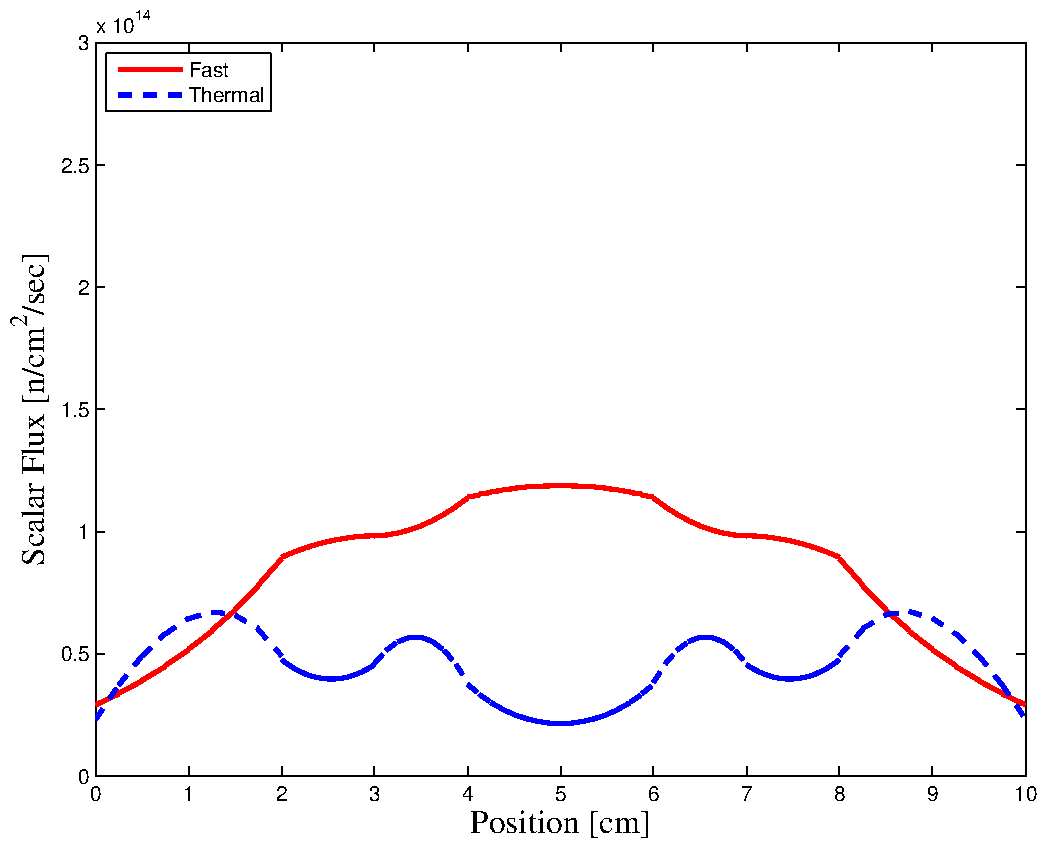
\includegraphics[width=11cm]{chapter5_depletion/P1_Lobatto_full_80_cells_t_steps60_End_600_Power_2000__BOC_Flux.pdf}
\caption{Example normalized scalar flux profiles at beginning and end of fuel burn-up cycle.}
\label{fig:ex_boc_cycle}
\end{figure}
%
\begin{figure}[!htp]
\centering
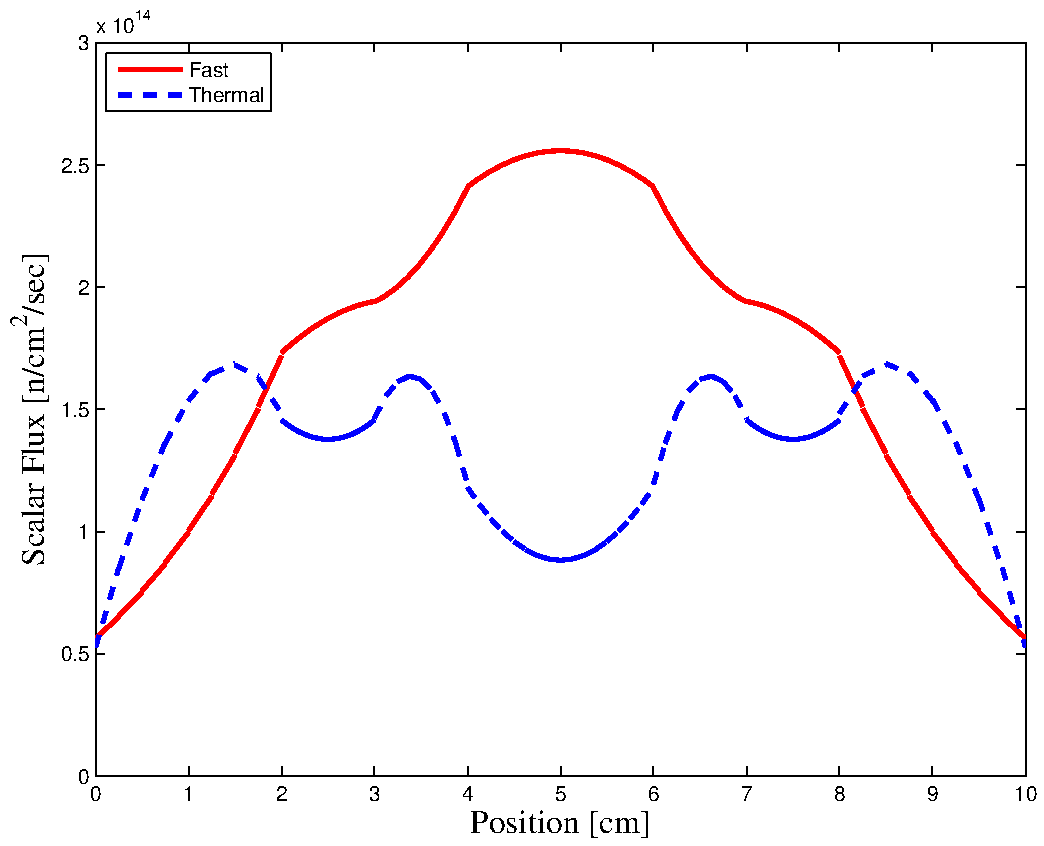
\includegraphics[width=11cm]{chapter5_depletion/P1_Lobatto_full_80_cells_t_steps60_End_600_Power_2000__EOC_Flux.pdf}
\caption{Example normalized scalar flux profiles at beginning and end of fuel burn-up cycle.}
\label{fig:ex_eoc_cycle}
\end{figure}

\section{Spatial Discretization}

We solve \eqts{eq:analytic_depletion} using a semi-static approach \cite{bell_glasstone} assuming the flux distribution at the start of the time step remains constant throughout the time step.
Nuclide densities are advanced in time using explicit Euler time differencing, then a corresponding radiation solution is found.  
We will consider three DFEM schemes to spatially discretize \eqts{eq:analytic_depletion}.
\begin{enumerate}
\item AD DFEM: expands the angular flux in a $P$ degree polynomial trial space using equally-spaced interpolation points, uses exact spatial integration, assumes  cell-wise constant cross sections for solving the radiation equations, and tracks only cell average nuclide densities.
\item SL Collapse: expands both the angular flux and nuclide densities in a $P$ degree polynomial trial space, uses self-lumping quadrature to approximate integrals, and assumes cell-wise constant cross sections for solving the radiation equations.
Lobatto quadrature is used as the DFEM interpolation points for odd degree trial spaces and Gauss quadrature as the DFEM interpolation points for even degree trial spaces.
\item SL Full: expands both the angular flux and nuclide densities in a $P$ degree polynomial trial space, uses self-lumping quadrature to approximate integrals, and explicitly accounts for the variation of macroscopic cross section within each spatial cell.
Lobatto quadrature is used as the DFEM interpolation points for odd degree trial spaces and Gauss quadrature as the DFEM interpolation points for even degree trial spaces.
\end{enumerate}

\subsection{Radiation Solution}

Using the nomenclature developed in Chapter \ref{sec:chapter2_constant_xs} and Chapter \ref{sec:chapter3_variable_xs}, the spatially discretized radiation equations are:
%The left hand sides of Eq. (\ref{eq:ss_depletion}a) and Eq. (\ref{eq:ss_depletion}b) are identical to the left hand side derived in \eqt{eq:mat_form} of \secref{sec:derive}.
%Noting that \eqt{eq:sn_def} holds not only for the analytic quantities, but also for numerical quantities, we introduce the numerical approximation to the group $g$ scalar flux, $\widetilde{\phi}_g(x)$:
%\benum
%\widetilde{\phi}_g(x) = \sum_{j=1}^{N_P}{\phi_{g,j} \B{j}(s)}
%\eenum 
\begin{multline}
\mu_d \mathbf{G} \vec{\psi}_{d,1} - \mu_d \psi_{in,d,1} \vec{f} + \R{\Sigma_{t,1}} \vec{\psi}_{d,1} = 
\frac{1}{4\pi}\R{\Sigma_{s,1\to1}}\vec{\phi}_1  \\
+ \frac{1}{k_{\tau}} \frac{1}{4\pi}\left( \R{\nu\Sigma_{f,1}} \vec{\phi}_1 +\R{\nu\Sigma_{f,2}} \vec{\phi}_2 \right)\pec 
\label{eq:fast_DFEM}
\end{multline}
%
and
%
\benum
\mu_d \mathbf{G} \vec{\psi}_{d,2} - \mu_d \psi_{in,d,2} \vec{f} + \R{\Sigma_{t,2}} \vec{\psi}_{d,2} = 
\frac{1}{4\pi}\left( \R{\Sigma_{s,2\to2}}\vec{\phi}_2  +
\R{\Sigma_{s,1\to2}}\vec{\phi}_1 \right) \pep
\label{eq:thermal_DFEM}
\eenum
In \eqt{eq:fast_DFEM} and \eqt{eq:thermal_DFEM} $k_{\tau}$ is the multiplication factor at time index $\tau$ and $\mathbf{R}_{\Sigma_{s,1\to1}}$, $\mathbf{R}_{\Sigma_{s,1\to2}}$, $\mathbf{R}_{\Sigma_{s,2\to2}}$, $\mathbf{R}_{\nu\Sigma_{f,1}}$, and $\mathbf{R}_{\nu\Sigma_{f,2}}$ are defined analogously to $\mathbf{R}_{\Sigma_t}$, as in \eqt{eq:chap3_react_mat}, replacing $\Sigma_t(s)$ with $\Sigma_{s,1\to1}(s)$, $\Sigma_{s,1\to2}(s)$, $\Sigma_{s,2\to2}(s)$, $\Sigma_{f,1}(s)$, and $\Sigma_{f,2}(s)$, respectively.

We solve \eqt{eq:fast_DFEM} and \eqt{eq:thermal_DFEM} following the standard power iteration procedure, described for DFEM neutron transport in 
\cite{warsa_k}.  
Convergence is checked after each power iteration.  
Using $\ell$ as the iteration index, convergence after the $\ell + 1$ iterate is said to occur when:
\benum
\delta_k = \abs{\frac{ k^{(\ell+1)} - k^{(\ell)}}{k^{(\ell)}}} < \epsilon_k \pec
\eenum
and
\benum
\delta_{\phi} = \max_{g=1,2}~~\max_{i=1,\dots,N_{cell}} ~~ \max_{j=1,\dots,N_P} ~~ \abs{ \frac{\phi_{g,i,j}^{(\ell+1)} - \phi_{g,i,j}^{(\ell)}}{\phi_{g,i,j}^{(\ell)}  } } < \epsilon_{\phi} \pep
\eenum
In our computational results we use $\epsilon_k = 10^{-12}$ and $\epsilon_{\phi} = 10^{-10}$.
For each power iteration, the within group components of \eqt{eq:fast_DFEM} and \eqt{eq:thermal_DFEM} are solved separately with a single transport sweep and S2SA iteration.
Since we are using an $S_2$ angular quadrature, a single source iteration with a single S2SA step exactly solves a given within group neutron transport problem.

The converged scalar flux is normalized such that the desired power level of $P_{Total} = 2000~[W/cm^2]$, is achieved.  
All fission energy is assumed to be deposited only in the fuel.
For the SL Full scheme, we calculate the normalization factor, $F_P$, as:
\benum
\label{eq:norm_F_sl_full}
F_P = E_f \sum_{g=1}^{2}{\left[ \sum_{i=1}^{N_{Fuel}}{ \frac{\Delta x_i}{2}\sum_{j=1}^{N_P}{ w_j \Sigma_{f,g,i,j} \phi_{g,i,j}    }}      \right]} \pec
\eenum
where in $E_f$ is the energy released per fission, assumed to be $200~[MeV]$, $w_j$ is the quadrature weight associated with the $j$-th DFEM interpolation point, and $N_{Fuel}$ is the total number of spatial cells in the fuel region.  
The SL Collapse and AD DFEM schemes calculate $F_P$ as
\benum
\label{eq:norm_F_udfem}
F_P = E_f \sum_{g=1}^2{
\left[ \sum_{i=1}^{N_{Fuel}}{ \frac{\Delta x_i \widehat{\Sigma}_{f,g,i}}{2}\sum_{j=1}^{N_P}{ w_j \Sigma_{f,g,i,j} \phi_{g,i,j}    }}      \right]
} \pep
\eenum
$\widetilde{\phi}^{(\ell+1)}$ is then scaled as:
\benum
\widetilde{\phi}_g^{(\ell+1)} \leftarrow \frac{P_{Total}}{F_P} \widetilde{\phi}_g^{(\ell+1)}   \pep
\eenum


%%%%%%%%%%%%%%%%%%%%%%%%%%%%%%%%%%%%%%%%%%%%%%%
\subsection{Nuclide Density}
%%%%%%%%%%%%%%%%%%%%%%%%%%%%%%%%%%%%%%%%%%%%%%%

We consider three spatial discretization schemes to solve the nuclide production/destruction components of \eqts{eq:analytic_depletion}.  
The first, AD DFEM, tracks only cell average nuclide densities, approximating the true spatial distribution of nuclide $m$, $N_m(x,t)$, as being a constant in each cell, equal to the cell average density of nuclide $m$.  
Denoting the average nuclide density in cell $i$ for nuclide $m$ as $\bar{N}_{m,i}$ and the average group $g$ scalar flux in cell $i$ as $\bar{\phi}_{g,i}$, we give the fissile nuclide update equation for the AD DFEM scheme in \eqt{eq:udfem_depletion}:
%\begin{subequations}
\begin{multline}
\frac{\bar{N}_{FS,i}^{\tau+1} - \bar{N}^{\tau}_{FS,i}}{\Delta t} = \bar{N}^{\tau}_{FT,i}\left[\gamma_{FT,1}\sigma_{a,FT,1} \bar{\phi}^{\tau}_{1,i} + \gamma_{FT,2}\sigma_{a,FT,2}\bar{\phi}^{\tau}_{2,i}  \right] \\
-\bar{N}^{\tau}_{FS,i}\left((1-\gamma_{FS,1})\sigma_{a,FS,1}\bar{\phi}^{\tau}_{1,i} + (1-\gamma_{FS,2})\sigma_{a,FS,2}\bar{\phi}^{\tau}_{2,i} \right) 
\pep
\label{eq:udfem_depletion}
\end{multline}
%
%
%\benum
%\frac{\bar{N}^{\tau+1}_{FT,i} - \bar{N}^{\tau}_{FT,i}}{\Delta t} = -\bar{N}^{\tau}_{FT,i}\left(\sigma_{a,FT,1}\bar{\phi}^{\tau}_{1,i} + \sigma_{a,FT,2}\bar{\phi}^{\tau}_{2,i}\right) 
%\eenum
%%
%%
%\begin{multline}
%\frac{\bar{N}_{FP-S,i}^{\tau+1} - \bar{N}^{\tau}_{FP-S,i}}{\Delta t} = 
%\bar{N}_{FT,i}^{\tau}\left[ (1-p_{FT,1})y_{FT}\sigma_{a,FT,1}\bar{\phi}^{\tau}_{1,i} \right] \\
%+\bar{N}_{FS,i}^{\tau} \left[ (1-p_{FS,1})y_{FS,1}\sigma_{a,FS,1}\bar{\phi}^{\tau}_{1,i} +  (1-p_{FS,2})y_{FS,2}\sigma_{a,FS,2}\bar{\phi}^{\tau}_{2,i} \right] \\
%- \bar{N}^{\tau}_{FS,i}\left[\sigma_{a,FP-S,1}\bar{\phi}_{1,i}^{\tau} + \sigma_{a,FP-S,2}\bar{\phi}_{2,i}^{\tau}  \right]
%\end{multline}
%%
%%
%%N_{fs}\int_0^{\inFTy}{\left[dE~(1-p_{fs})y_{fs}\sigma_{a,fs} \phi\right]} + 
%%N_{FT}\int_0^{\inFTy}{\left[dE~ (1-p_{FT}) y_{FT} \sigma_{a,FT} \phi \right]} \\
%%
%%
%
%\begin{multline}
%\frac{\bar{N}_{FP-A,i}^{\tau+1} - \bar{N}^{\tau}_{FP-A,i}}{\Delta t} = 
%\bar{N}_{FT,i}^{\tau} p_{FT,1} y_{FT,1}\sigma_{a,FT,1}\bar{\phi}^{\tau}_{1,i} \\
% + \bar{N}_{FS,i}^{\tau}\left[ p_{FS,1} y_{FS,1} \sigma_{a,FS,1}\bar{\phi}^{\tau}_{1,i} + p_{FS,2} y_{FS,2} \sigma_{a,FS,2}\bar{\phi}^{\tau}_{2,i}  \right] \\
%- \bar{N}_{FP-A,i}^{\tau}\left[ (1-\xi_{FP-A,1})\sigma_{a,FP-A,1}\bar{\phi}_{1,i}^{\tau} + (1-\xi_{FP-A,2})\sigma_{a,FP-A,2}\bar{\phi}_{2,i}^{\tau}  \right] 
%\end{multline}
%%N_{fs}\int_0^{\inFTy}{\left[dE~p_{fs} y_{fs} \sigma_{a,fs} \phi \right]} + 
%%N_{FT} \int_0^{\inFTy}{\left[dE~p_{FT} y_FT\sigma_{a,FT} \phi\right]} - 
%%N_{FP-A}\int_0^{\inFTy}{\left[ dE~ (1-\xi_{FP-A})\sigma_{a,FP-A}  \phi \right]}   \\
%%
%%
%\begin{multline}
%\frac{ \bar{N}_{I,i}^{\tau+1} - \bar{N}^{\tau}_{I,i}}{\Delta t} = 
% \bar{N}^{\tau}_{FP-S,i}\left[ \sigma_{a,FP-S,1}\bar{\phi}^{\tau}_{1,i} + \sigma_{a,FP-S,2}\bar{\phi}^{\tau}_{2,i}  \right] + \\
% \bar{N}_{FP-A,i}^{\tau} \left[  \xi_{FP-A,1}\sigma_{a,FP-A,1}\bar{\phi}^{\tau}_{1,i} + \xi_{FP-A,2}\sigma_{a,FP-A,2}\bar{\phi}^{\tau}_{2,i} \right] \pec
%\end{multline}
%\end{subequations}
In \eqt{eq:udfem_depletion} superscript $\tau$ denotes time index $\tau$ quantities and $\Delta t$ is the time step size.
The update equations for $N_{FT}$, $N_{FP-A}$, $N_{FP-S}$, and $N_I$ can be derived analogously to \eqt{eq:udfem_depletion}.
AD DFEM calculates $\bar{\phi}_{g,i}$ using closed Newton-Cotes quadrature with the quadrature points limited to the DFEM interpolation points:
\benum
\label{eq:avg}
\bar{\phi}_{g,i} = \frac{1}{2}\sum_{j=1}^{N_P}{w_j \phi_{g,j} } \pep
\eenum
The averaging in \eqt{eq:avg} is exact since an $N_P$ point closed Newton-Cotes quadrature can exactly integrate any $P$ degree polynomial.
Equation (\ref{eq:udfem_depletion}) locally updates all average nuclide densities, $\bar{N}_{FS,i},~\bar{N}_{FT,i},~\bar{N}_{FP-A,i},~\bar{N}_{FP-S,i},~\text{and} \bar{N}_{I,i}$, simultaneously via a $5\times5$ matrix-vector multiply.

The SL Full and SL Collapse schemes approximate the true spatial density of nuclide $m$ as a $P$ degree Lagrange polynomial, $\widetilde{N}_m(s)$, in each cell:
\benum
\widetilde{N}_m(s) = \sum_{j=1}^{N_P}{N_{m,j} \B{j}(s)} \pec
\label{eq:nuc_m_unk}
\eenum
where \B{j} are the $N_P = P+1$  Lagrange interpolatory polynomials in the interval $s\in[-1,1]$.  
We require the set of nuclide density DFEM interpolation points to be the same set of $N_P$ points as the angular flux DFEM interpolation points.
Following a Galerkin procedure, we multiply each production/destruction nuclide equation of \eqts{eq:analytic_depletion} by basis function $\B{j}$ and integrate generating  $5(P+1)$ equations.
The system of update equations for $\vec{N}_{FS,i}$ is shown in \eqts{eq:dfem_nuclide}:
%\begin{subequations}
\begin{multline}
\frac{1}{\Delta t}\M\left(\vec{N}_{FS,i}^{\tau+1} - \vec{N}_{FS,i}^{\tau} \right) = -(1-\gamma_{FS,1})\sigma_{a,FS,1}\Mw_{\phi_{1,i},\tau}\vec{N}_{FS,i}^{\tau} \\
- (1-\gamma_{FS,2})\sigma_{a,FS,2}\Mw_{\phi_{2,i},\tau}\vec{N}_{FS,i}^{\tau} \\
+ \gamma_{FT,1}\sigma_{a,FT,1}\Mw_{\phi_{1,i}^{\tau}}\vec{N}_{FT,i}^{\tau}  + \gamma_{FT,2}\sigma_{a,FT,2}\Mw_{\phi_{2,i}^{\tau}}\vec{N}_{FT,i}^{\tau} 
\pep
\label{eq:dfem_nuclide}
\end{multline}
%
%%
%\benum
%\frac{1}{\Delta t}\M\left(\vec{N}_{FT,i}^{\tau+1} - \vec{N}_{FT,i}^{\tau} \right) = 
%-\sigma_{a,FT,1}\Mw_{\phi_{1,i}^{\tau}}\vec{N}_{FT,i}^{\tau} - \sigma_{a,FT,2}\Mw_{\phi_{2,i}^{\tau}}\vec{N}_{FT,i}^{\tau}
%\eenum
%%
%%
%\begin{multline}
%\frac{1}{\Delta t}\M\left(\vec{N}_{FP-S,i}^{\tau+1} - \vec{N}_{FP-S,i}^{\tau}\right) =  (1-p_{FS,1})y_{FS,1}\sigma_{a,FS,1}\Mw_{\phi_{1,i}^{\tau}}\vec{N}_{FS,i}^{\tau} \\ 
%+  (1-p_{FS,2})y_{FS,2}\sigma_{a,FS,2}\Mw_{\phi_{2,i}^{\tau}}\vec{N}_{FP-S,i}^{\tau} 
%+ (1-p_{FT,1})y_{FT}\sigma_{a,FT,1}\Mw_{\phi_{1,i}^{\tau}}\vec{N}_{FT,i}^{\tau}  \\
%- \sigma_{a,FP-S,1}\Mw_{\phi_{1,i}^{\tau}}\vec{N}_{FS,i}^{\tau} - \sigma_{a,FP-S,2}\Mw_{\phi_{2,i}^{\tau}}\vec{N}_{FS,i}^{\tau}
%\end{multline}
%%
%%
%%N_{fs}\int_0^{\inFTy}{\left[dE~(1-p_{fs})y_{fs}\sigma_{a,fs} \phi\right]} + 
%%N_{FT}\int_0^{\inFTy}{\left[dE~ (1-p_{FT}) y_{FT} \sigma_{a,FT} \phi \right]} \\
%%
%%
%
%\begin{multline}
%\frac{1}{\Delta t}\M\left(\vec{N}_{FP-A,i}^{\tau+1} - \vec{N}_{FP-A,i}^{\tau}\right) =   p_{FT,1} y_{FT,1}\sigma_{a,FT,1}\Mw_{\phi_{1,i}^{\tau}}\vec{N}_{FT,i}^{\tau}  \\
%+ p_{FS,1} y_{FS,1} \sigma_{a,FS,1}\Mw_{\phi_{1,i}^{\tau}}\vec{N}_{FS,i}^{\tau} 
%+ p_{FS,2} y_{FS,2} \sigma_{a,FS,2} \Mw_{\phi_{2,i}^{\tau}} \vec{N}_{FS,i}^{\tau}  \\
%- (1-\xi_{FP-A,1})\sigma_{a,FP-A,1}\Mw_{\phi_{1,i}^{\tau}}\vec{N}_{FP-A,i}^{\tau} \\
%- (1-\xi_{FP-A,2})\sigma_{a,FP-A,2}\Mw_{\phi_{2,i}^{\tau}}\vec{N}_{FP-A,i}^{\tau}  
%\end{multline}
%%N_{fs}\int_0^{\inFTy}{\left[dE~p_{fs} y_{fs} \sigma_{a,fs} \phi \right]} + 
%%N_{FT} \int_0^{\inFTy}{\left[dE~p_{FT} y_FT\sigma_{a,FT} \phi\right]} - 
%%N_{FP-A}\int_0^{\inFTy}{\left[ dE~ (1-\xi_{FP-A})\sigma_{a,FP-A}  \phi \right]}   \\
%%
%%
%\begin{multline}
%\frac{1}{\Delta t}\M \left(\vec{N}_{I,i}^{\tau+1} - \vec{N}_{I,i}^{\tau}\right) = 
%\xi_{FP-A,1}\sigma_{a,FP-A,1}\Mw_{\phi_{1,i}^{\tau}}\vec{N}_{FP-A,i}^{\tau} \\
%+ \xi_{FP-A,2}\sigma_{a,FP-A,2}\Mw_{\phi_{2,i}^{\tau}}\vec{N}_{FP-A,i}^{\tau} 
% \\
%+ \sigma_{a,FP-S,1}\Mw_{\phi_{1,i}^{\tau}}\vec{N}_{FP-S,i}^{\tau} + \sigma_{a,FP-S,2}\Mw_{\phi_{2,i}^{\tau}}\vec{N}_{FP-S,i}^{\tau} \pec
%\end{multline}
%\end{subequations}
The equations for $\vec{N}_{FT,i}$, $\vec{N}_{FP-A,i}$, $N_{FP-S,i}$, and $N_{I,i}$ are derived in a similar fashion to \eqt{eq:dfem_nuclide}.  
In \eqt{eq:dfem_nuclide} we have defined:
\benum
\Mw_{\phi_{g,i}^{\tau},jk} = \frac{\Delta x}{2}\int_{-1}^{1}{\B{j}(s)\B{k}(s)\widetilde{\phi}_{g,\tau,i}(s)~ds} ~~\text{, and}
\label{eq:mw_mat}
\eenum
\benum
\vec{N}_{m,i}^{\tau} = \left[ \begin{array}{c}
N_{m,1}^{\tau}  \\
\vdots \\
N_{m,j}^{\tau}  \\
\vdots \\
N_{m,P+1}^{\tau} 
\end{array} \right]
 \pep
\eenum
Given that we track five nuclides in the fuel region, each expanded in a $P$ degree polynomial in each cell, there are $5(P+1)$ unknowns in each cell, thus \eqt{eq:dfem_nuclide} is a closed, $5(P+1) \times 5(P+1)$ system of linear equations for the $5(P+1)$ unknown nuclide densities, $N_{m,i,j}$ in each cell.
%
%Solution of \eqts{eq:dfem_nuclide} can be simplified by defining two matrices, $\mathbf{G}_1$ and $\mathbf{G}_2$:
%\benum
%\label{eq:g_mat}
%\mathbf{G}_g = \M^{-1}\Mw_{\phi_{g,\tau,i}} \pec
%\eenum
%requiring only two $N_P \times N_P$ matrix inversions rather than one for each nuclide tracked.
%
%then all of the nuclide density unknowns in \eqts{eq:dfem_nuclide} can be solved by inverting only two $P+1 \times P+1$ matrices and using matrix vector multiplication to find all $\vec{N}_{m,\tau+1}$.  
%For brevity, we omit these equations, as they are readily apparent when \eqt{eq:dfem_nuclide} is solved for $\vec{N}_{m,\tau+1}$, and the definition of \eqt{eq:g_mat} is applied.
%With SL Full and SL Collapse schemes, \M and $\Mw_{\phi,\tau,g}$ of \eqts{eq:dfem_nuclide} are diagonal matrices, and the number of nuclides is very small, so the benefit of calculating $\mathbf{G}_g$ is minimal.  
%If we considered a more realistic number of nuclides, or if \M was a dense matrix, then the use of $\mathbf{G}_g$ would be essential for minimizing computational cost.

Using self-lumping quadrature to approximate \eqt{eq:mw_mat} causes $\Mw_{\phi_{g,i}^{\tau}}$ to be a diagonal matrix.  
Recalling that $\widetilde{N}_m$ uses the same interpolation points as $\widetilde{\phi}_g$, approximating the integration of \eqt{eq:mw_mat} with numerical quadrature restricted to the DFEM interpolating points, results in
\benum
\Mw_{\phi_{g,i}^{\tau},jk} = \left \{ 
\begin{array}{ll} 
w_j \frac{\Delta x}{2} \phi_{g,\tau,i,j} & j=k \\
0 & \text{otherwise} 
\end{array}
\right. \pep
\eenum

Macroscopic cross sections are generated from nuclide density and microscopic cross section data.
%s $[b]$, $1b = 10^{-24}~cm^2$, by multiplying a given nuclide's density by the microscopic cross section of that nuclide for a specific reaction, and then summing over all nuclides.  
For the AD DFEM scheme, each cell has a single macroscopic cross section (per reaction type), and a single value of nuclide density for each nuclide type.  
Thus, interaction cross sections are easily tabulated.  As an example, the cell average total interaction cross section in cell $i$ is calculated in \eqt{eq:udfem_sigt}:
\begin{multline}
\widehat{\Sigma}_{t,g,i} = N_{FS,i}\sigma_{t,FS,g} + N_{FT,i}\sigma_{t,FT,g} + N_{FP-A,i}\sigma_{t,FP-A,g} 
\\ + N_{FP-S,i}\sigma_{t,FP-S,g} + N_{I,i}\sigma_{t,I,g} \pep
\label{eq:udfem_sigt}
\end{multline}
Macroscopic fission cross section and average neutrons per fission products are found in a similar fashion, but we can limit our consideration to the fissile and fertile nuclide densities as shown in \eqt{eq:udfem_sigf},
\benum
\label{eq:udfem_sigf}
\widehat{\nu\Sigma}_{f,g,i} = N_{FS,i}\nu_{FS,g}\sigma_{f,FS,g} +  N_{FT,i}\nu_{FT,g}\sigma_{f,FT,g}  \pep
\eenum
The SL Full and SL Collapse schemes calculate macroscopic cross sections in a similar fashion to \eqt{eq:udfem_sigt} and \eqt{eq:udfem_sigf}, but instead of calculating a cell average, $\widehat{\Sigma}_{g,i}$, they calculate macroscopic values at each DFEM interpolation point.
%\benum
%\label{eq:sl_xs}
%\Sigma_{t,g,i,j} = N_{FS,i,j}\sigma_{t,FS,g} + N_{FT,i,j}\sigma_{t,FT,g} + N_{FP-A,i,j}\sigma_{t,FP-A,g} + N_{FP-S,i,j}\sigma_{t,FP-S,g} + N_{I,i,j}\sigma_{t,I,g}
%\pep
%\eenum
SL Collapse then averages the macroscopic cross section at each DFEM interpolation point to estimate the cell average cross section, as shown in \eqt{eq:xs_averaging} for  $\widehat{\Sigma}_{t,i}$: 
\benum
\widehat{\Sigma}_{t,i} = \frac{1}{2}\sum_{j=1}^{N_P}{w_j \Sigma_{t,g,i,j}} \pep
\label{eq:xs_averaging}
\eenum

%%%%%%%%%%%%%%%%%%%%%%%%%%%%%%%%%%%%%%%%%%%%%%%%%%%%%%%%%%%%%%%%%%%%%
\section{Numerical Results}
%%%%%%%%%%%%%%%%%%%%%%%%%%%%%%%%%%%%%%%%%%%%%%%%%%%%%%%%%%%%%%%%%%%%%

Since an analytic solution to this depletion problem is not available we employ a fine spatial mesh to obtain the reference solution.  
We use a fine mesh of 10,240 cells and the SL Full scheme with a quartic polynomial trial space as our reference numerical solution. 
%Our results demonstrate that the SL Full scheme using a quartic polynomial DFEM trial space is the most accurate scheme.   
We present $L_2$ spatial error measures for 
\begin{enumerate}
\item the total scalar flux ($E_{\phi}$), 
\item the fissile nuclide density ($E_{N_{FS}}$),
\item the fertile nuclide density ($E_{N_{FT}}$), and 
\item the parasitic absorber fission product ($E_{N_{FP-A}}$).
\end{enumerate}
To allow for easier comparison, we normalize each error to the reference solution quantity.
We define $E_{\phi}$ as:
\benum
E_{\phi} = \frac{\sqrt{\sum_{g=1}^2{\sum_{i=1}^{N_{ref}}{ \frac{\Delta x_i}{2} \sum_{q=1}^{N_{qf}}{ w_q\left( \widetilde{\phi}_{ref,i,g}(s_q) - \widetilde{\phi}_{num,i,g}(s_q)  \right)^2}}}}}{\sqrt{\sum_{g=1}^2{\sum_{i=1}^{N_{ref}}{ \frac{\Delta x_i}{2} \sum_{q=1}^{N_{qf}}{ w_q\widetilde{\phi}_{ref,i,g}(s_q)^2  }}}}} \pec
\eenum
%
%
%%%E_{N_{FS}} &=& \frac{\sqrt{\sum_{i=1}^{N_{ref}}{ \frac{\Delta x_i}{2} \sum_{q=1}^{N_{qf}}{ w_q\left( \widetilde{N}_{FS,ref,i}(s_q) - \widetilde{N}_{FS,num,i}(s_q)  \right)^2}}}}{\sqrt{\sum_{i=1}^{N_{ref}}{ \frac{\Delta x_i}{2} \sum_{q=1}^{N_{qf}}{ w_q\widetilde{N}_{FS,ref,i}(s_q)^2  }}}} \pec \\
%%%%
%%%%
%%%E_{N_{FT}} &=& \frac{\sqrt{\sum_{i=1}^{N_{ref}}{ \frac{\Delta x_i}{2} \sum_{q=1}^{N_{qf}}{ w_q\left( \widetilde{N}_{FT,ref,i}(s_q) - \widetilde{N}_{FT,num,i}(s_q)  \right)^2}}}}{\sqrt{\sum_{i=1}^{N_{ref}}{ \frac{\Delta x_i}{2} \sum_{q=1}^{N_{qf}}{ w_q\widetilde{N}_{FT,ref,i}(s_q)^2  }}}} \pec \\
%%%%
%%%%
%%%E_{N_{FP-A}} &=& \frac{\sqrt{\sum_{i=1}^{N_{ref}}{ \frac{\Delta x_i}{2} \sum_{q=1}^{N_{qf}}{ w_q\left( \widetilde{N}_{FP-A,ref,i}(s_q) - \widetilde{N}_{FP-A,num,i}(s_q)  \right)^2}}}}
%%%{\sqrt{\sum_{i=1}^{N_{ref}}{ \frac{\Delta x_i}{2} \sum_{q=1}^{N_{qf}}{ w_q\widetilde{N}_{FP-A,ref,i}(s_q)^2  }}}} \pep
%%%\eeanum
where $N_{ref}$ is the number of reference cells, $\widetilde{\phi}_{ref,i,g}(s)$ is the reference solution group $g$ scalar flux in cell $i$, and $\widetilde{\phi}_{num,i,g}(s)$ is the coarse mesh numerical scheme's approximation of the group $g$ scalar flux in cell $i$.
Error measures for $N_{FS}$, $N_{FT}$, and $N_{FP-A}$ are derived similarly.

Convergence of $E_{\phi}$ is shown in \figs{fig:depletion_flux_p1}{fig:depletion_flux_p4} as a function of DFEM trial space degree and DFEM scheme.
\begin{figure}[!hbp]
\centering
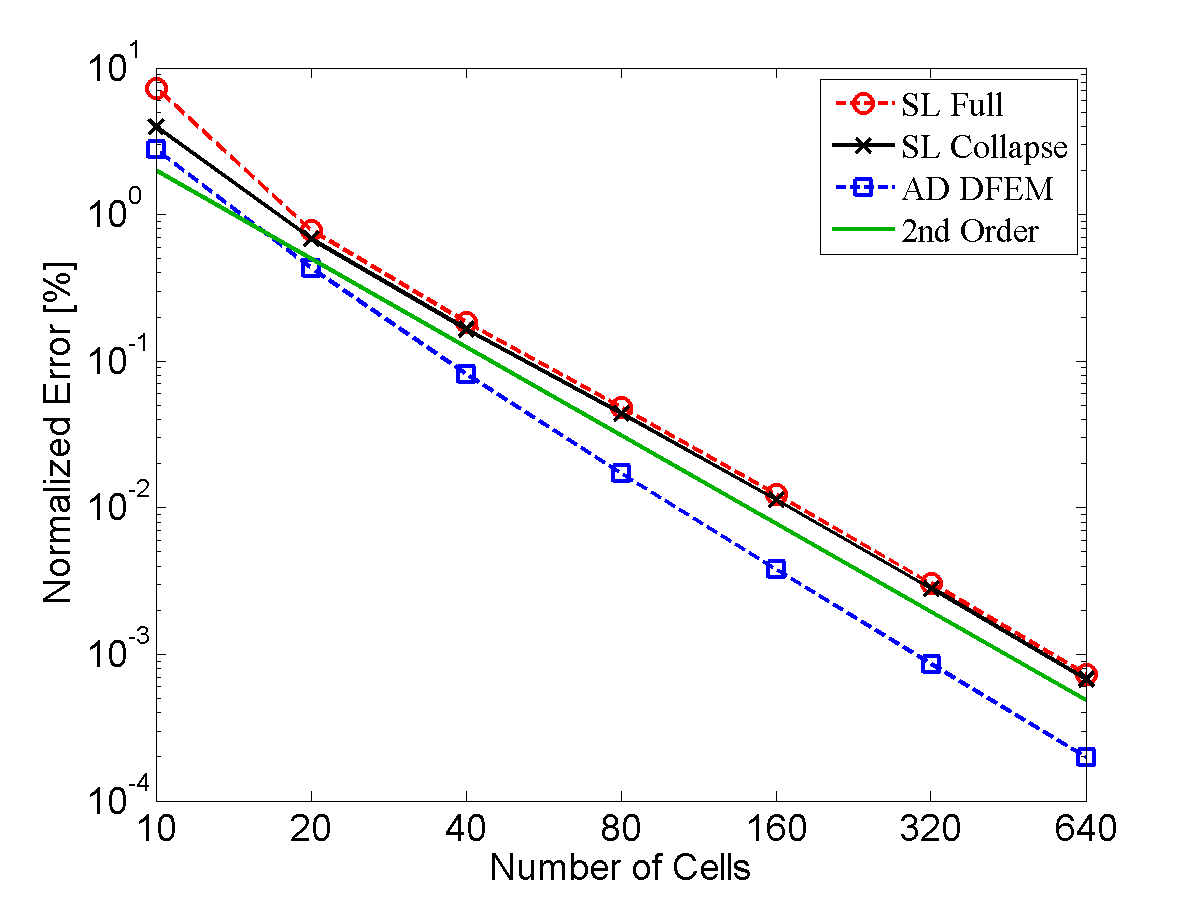
\includegraphics[width=9.5cm]{chapter5_depletion/Flux_P1_norm_err.png}
\caption{Normalized total scalar flux error for the depletion problem at end of cycle, for linear DFEM.}
\label{fig:depletion_flux_p1}
\end{figure}

\pagebreak

\begin{figure}[!htp]
\centering
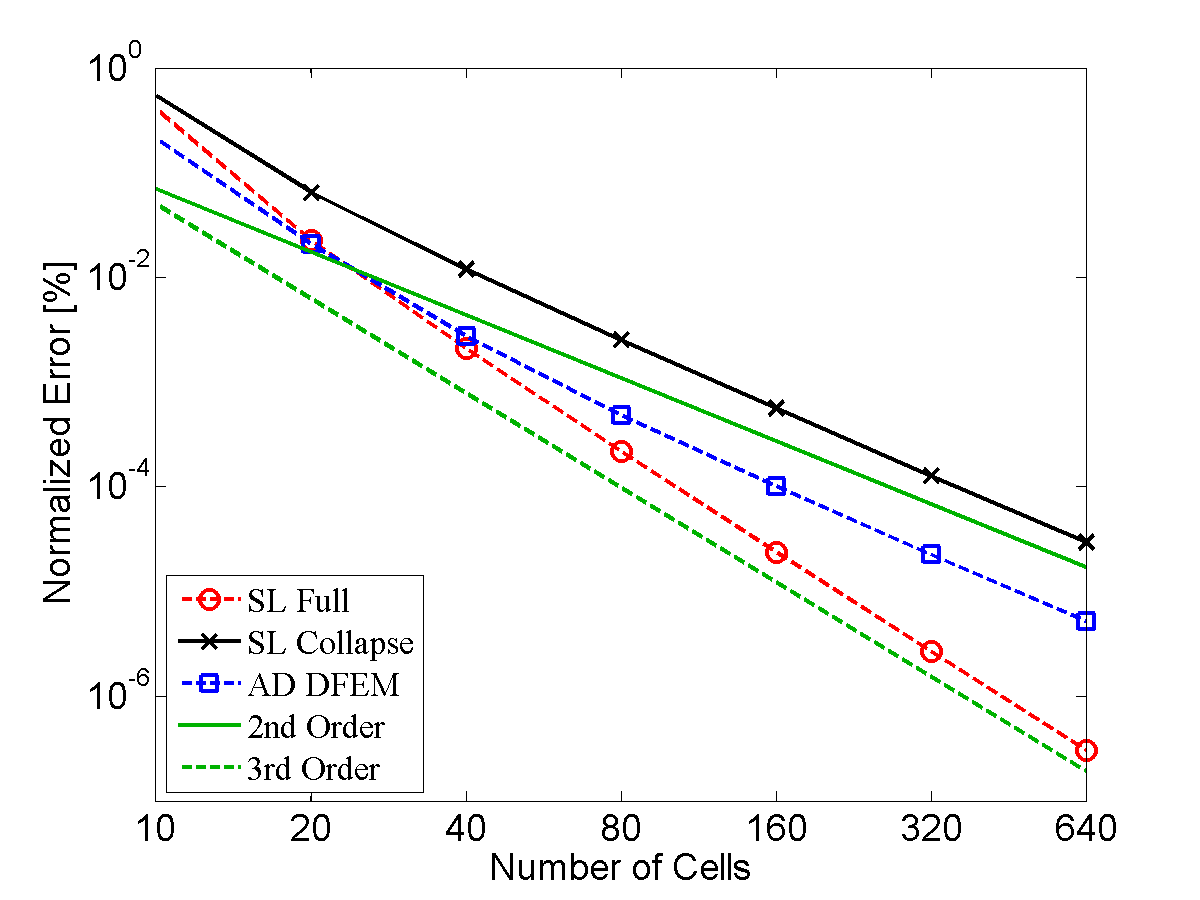
\includegraphics[width=9.5cm]{chapter5_depletion/Flux_P2_norm_err.png}
\caption{Normalized total scalar flux error for the depletion problem at end of cycle, for quadratic DFEM.}
\label{fig:depletion_flux_p2}
\end{figure}

\begin{figure}[!hbp]
\centering
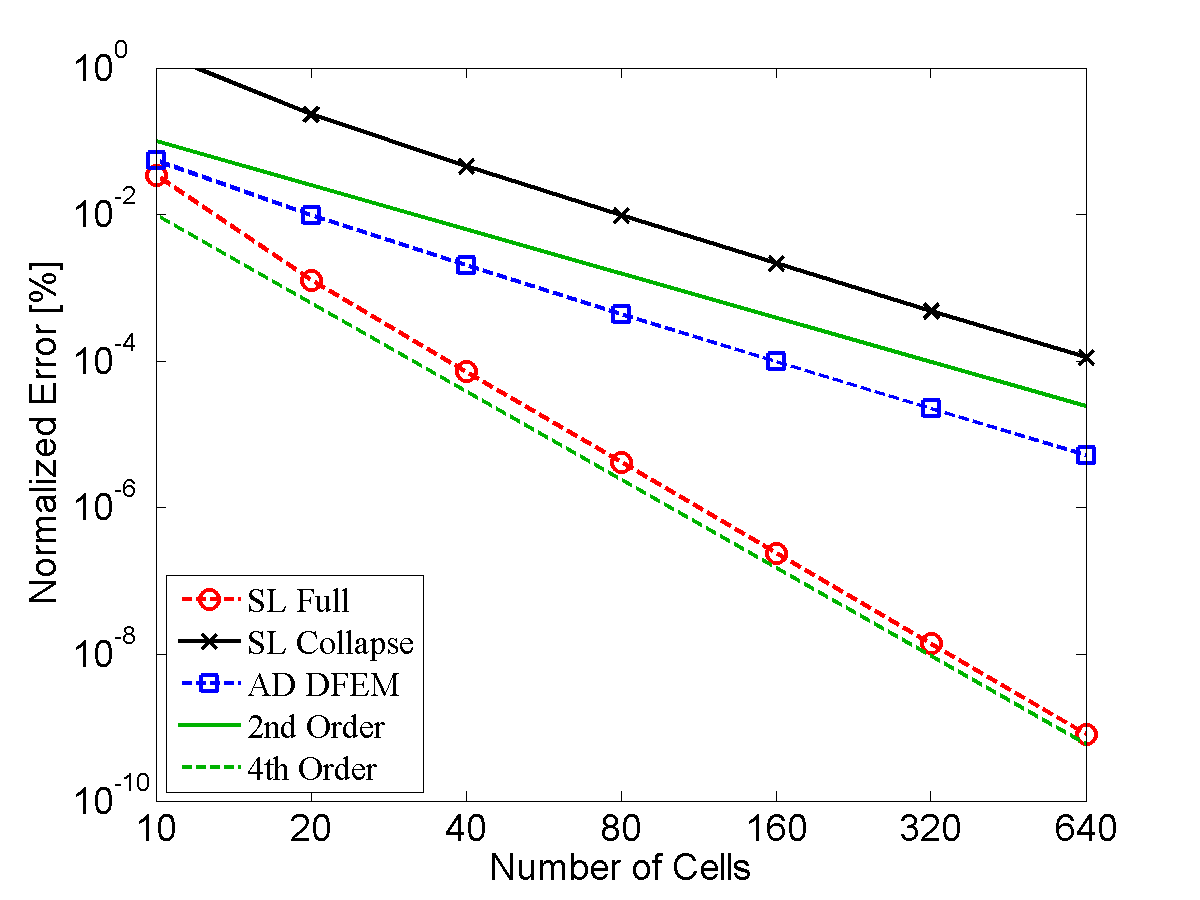
\includegraphics[width=9.5cm]{chapter5_depletion/Flux_P3_norm_err.png}
\caption{Normalized total scalar flux error for the depletion problem at end of cycle, for cubic DFEM.}
\label{fig:depletion_flux_p3}
\end{figure}

\pagebreak

\begin{figure}[!htp]
\centering
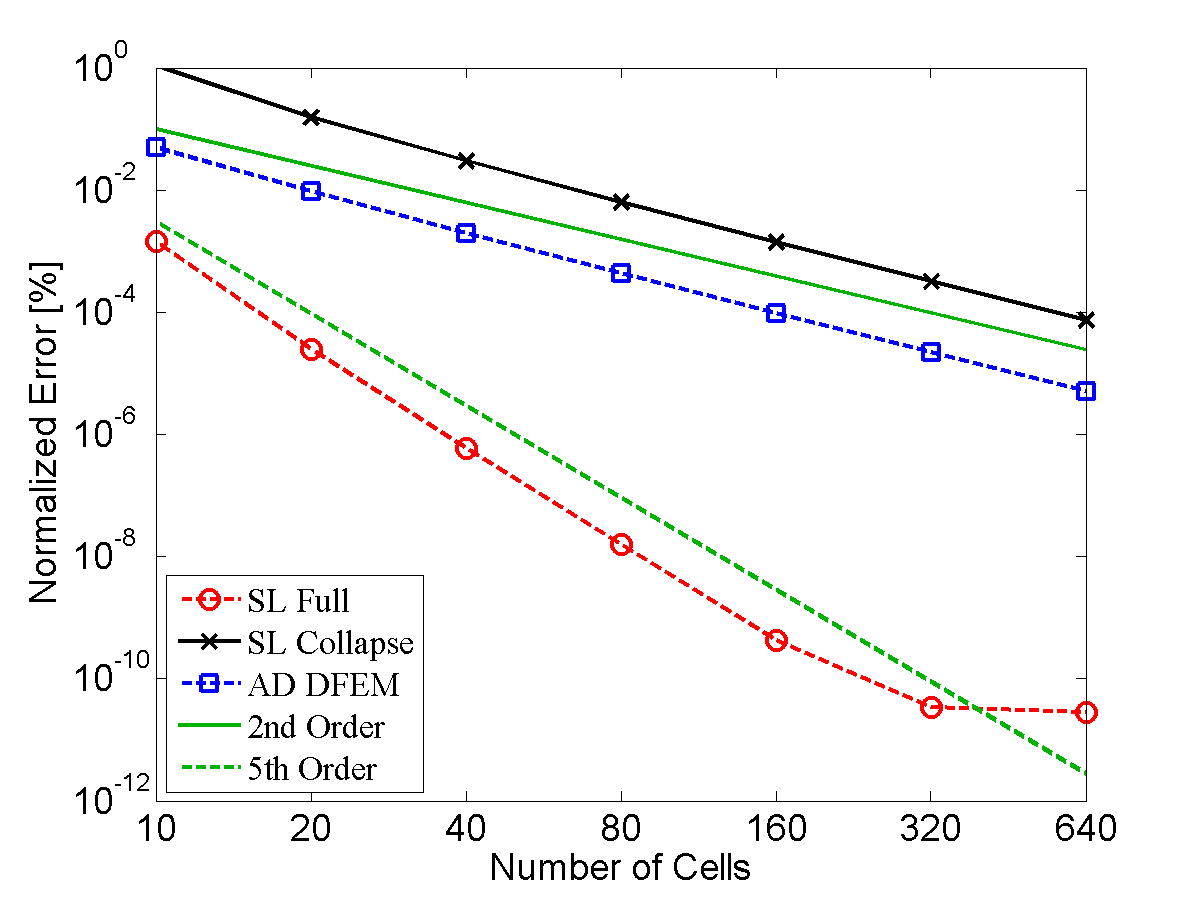
\includegraphics[width=9.5cm]{chapter5_depletion/Flux_P4_norm_err.png}
\caption{Normalized total scalar flux error for the depletion problem at end of cycle, for quartic DFEM.}
\label{fig:depletion_flux_p4}
\end{figure}

Figures \ref{fig:depletion_flux_p1}-\ref{fig:depletion_flux_p4} re-emphasize two key results observed in the case of a pure absorber.
First, when employing cell-wise constant cross sections, angular / scalar flux convergence is at most second order in space, regardless of the DFEM trial space polynomial degree.
Second, exact integration of the interaction terms in the DFEM moment equations is not required to achieve high-order accuracy.
In the depletion term, the DFEM interaction term is a degree $3P$ polynomial, and self-lumping schemes using Gauss or Lobatto quadrature only integrate $2P+1$ and $2P-1$ degree polynomials, respectively.

Convergence of $E_{N_{FS}}$, $E_{N_{FT}}$, and $E_{N_{FP-A}}$ are given in 
\figs{fig:depletion_NFS_p1}{fig:depletion_NFS_p4}, \figs{fig:depletion_NFT_p1}{fig:depletion_NFT_p4}, and \figs{fig:depletion_NFPA_p1}{fig:depletion_NFPA_p4}, respectively for linear through quartic trial space degrees.

\begin{figure}[!htp]
\centering
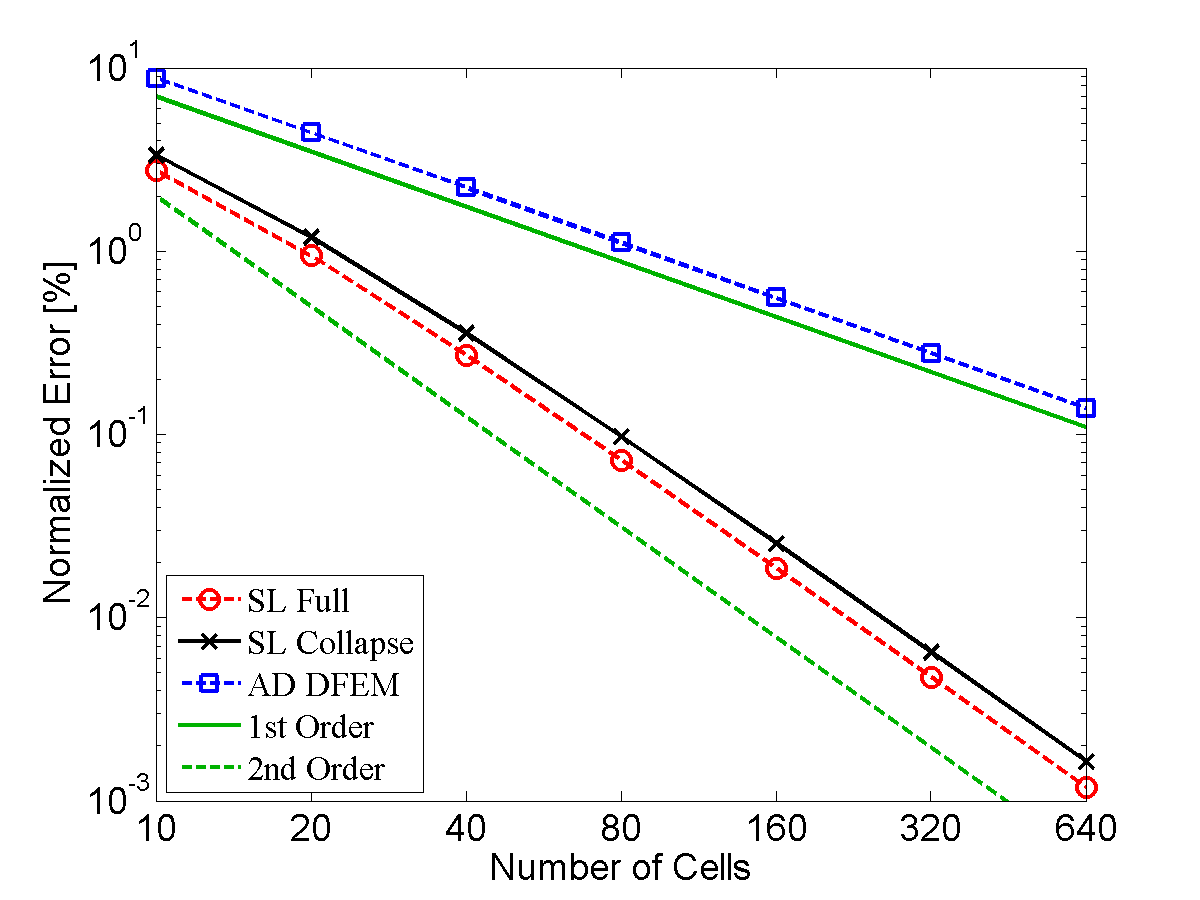
\includegraphics[width=9.5cm]{chapter5_depletion/FS_P1_norm_err.png}
\caption{Normalized fissile nuclide density error for the depletion problem at end of cycle, for linear DFEM}
\label{fig:depletion_NFS_p1}
\end{figure}

\begin{figure}[!hbp]
\centering
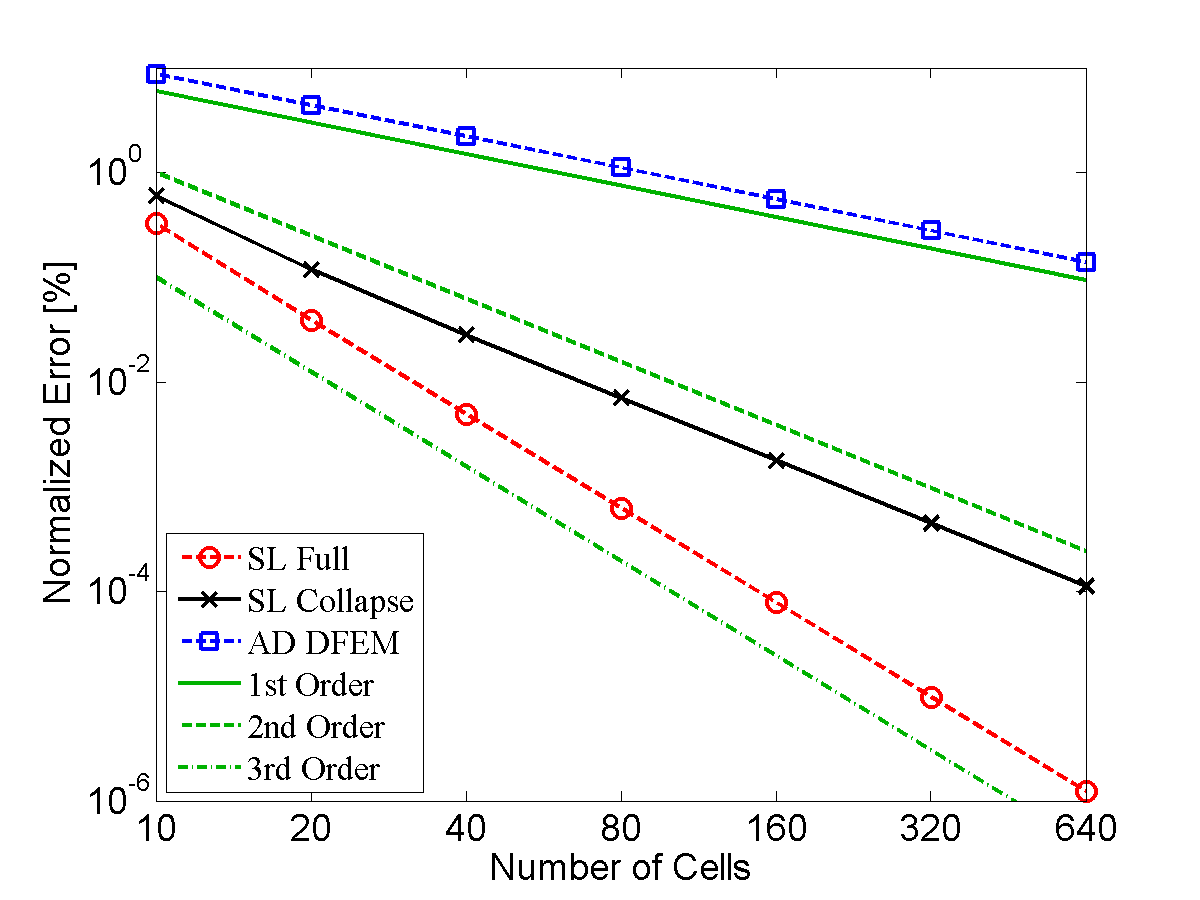
\includegraphics[width=9.5cm]{chapter5_depletion/FS_P2_norm_err.png}
\caption{Normalized fissile nuclide density error for the depletion problem at end of cycle, for quadratic DFEM.}
\label{fig:depletion_NFS_p2}
\end{figure}

\begin{figure}[!htp]
\centering
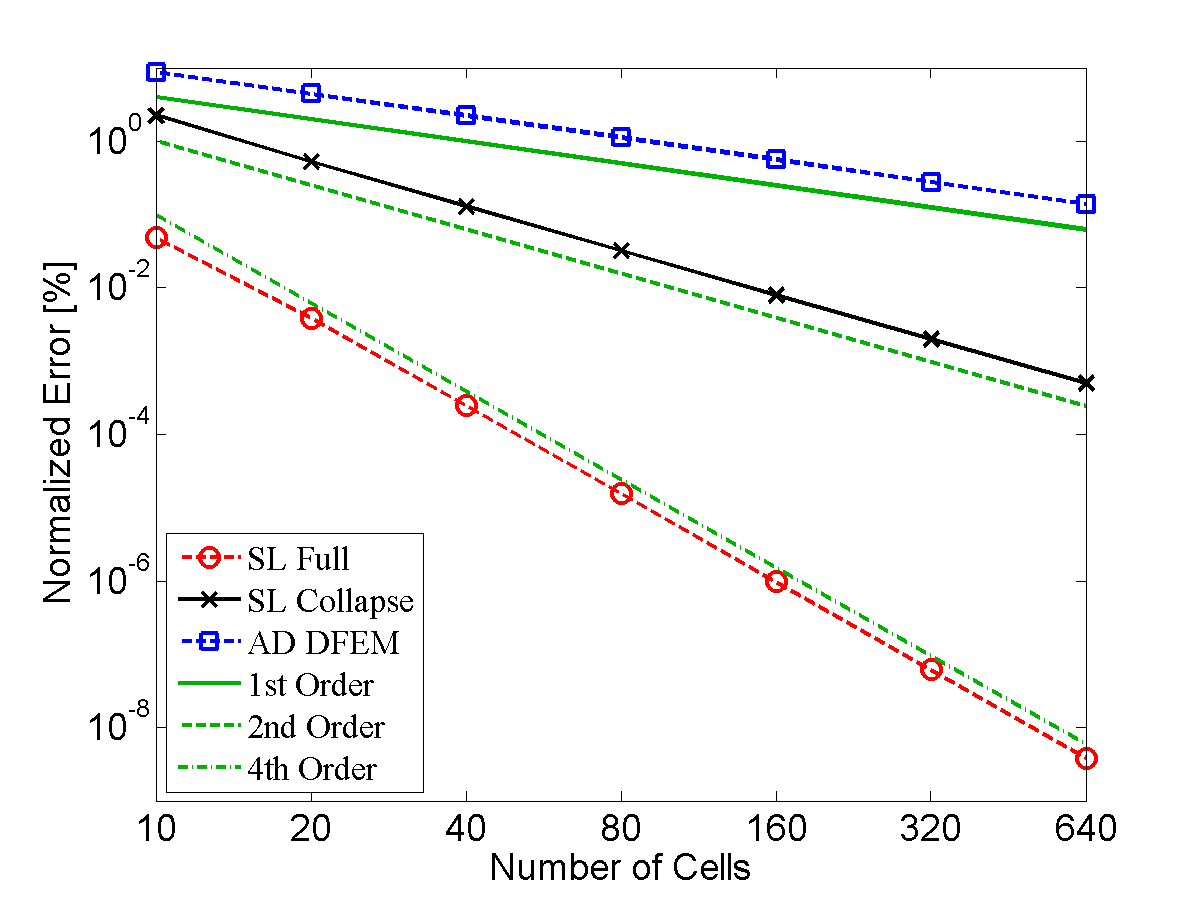
\includegraphics[width=9.5cm]{chapter5_depletion/FS_P3_norm_err.png}
\caption{Normalized fissile nuclide density error for the depletion problem at end of cycle, for cubic DFEM.}
\label{fig:depletion_NFS_p3}
\end{figure}

\begin{figure}[!hbp]
\centering
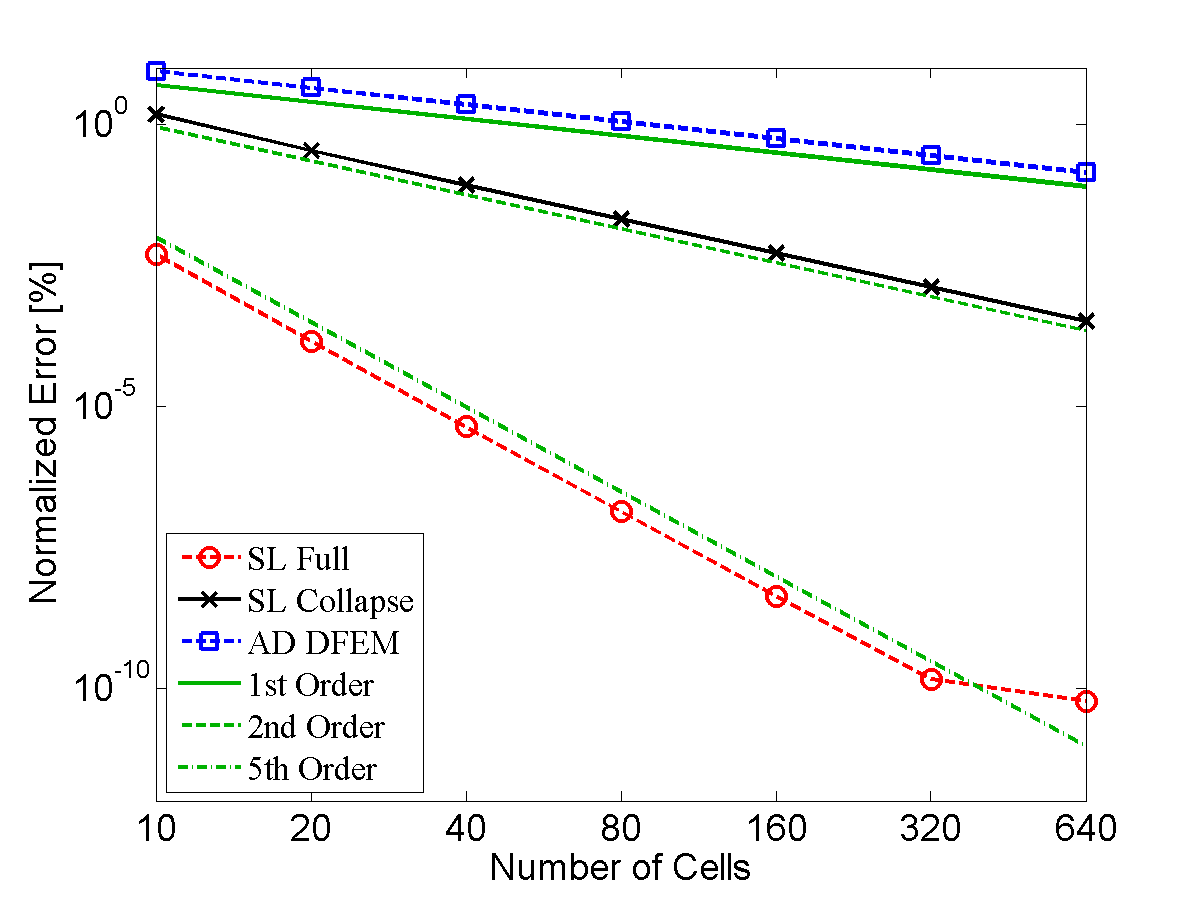
\includegraphics[width=9.5cm]{chapter5_depletion/FS_P4_norm_err.png}
\caption{Normalized fissile nuclide density error for the depletion problem at end of cycle, for quartic DFEM.}
\label{fig:depletion_NFS_p4}
\end{figure}

\pagebreak

\begin{figure}[!htp]
\centering
\includegraphics[width=9.5cm]{chapter5_depletion/ft_P1_norm_err.png}
\caption{Normalized fertile nuclide density error for the depletion problem at end of cycle, for linear DFEM.}
\label{fig:depletion_NFT_p1}
\end{figure}
%
\begin{figure}[!hbp]
\centering
\includegraphics[width=9.5cm]{chapter5_depletion/ft_P2_norm_err.png}
\caption{Normalized fertile nuclide density error for the depletion problem at end of cycle, for quadratic DFEM..}
\label{fig:depletion_NFT_p2}
\end{figure}
%
\newpage
%
\begin{figure}[!htp]
\centering
\includegraphics[width=9.5cm]{chapter5_depletion/ft_P3_norm_err.png}
\caption{Normalized fertile nuclide density error for the depletion problem at end of cycle, for cubic DFEM.}
\label{fig:depletion_NFT_p3}
\end{figure}

\begin{figure}[!hbp]
\centering
\includegraphics[width=9.5cm]{chapter5_depletion/ft_P4_norm_err.png}
\caption{Normalized fertile nuclide density error for the depletion problem at end of cycle, for quartic DFEM.}
\label{fig:depletion_NFT_p4}
\end{figure}

\newpage

\begin{figure}[!htp]
\centering
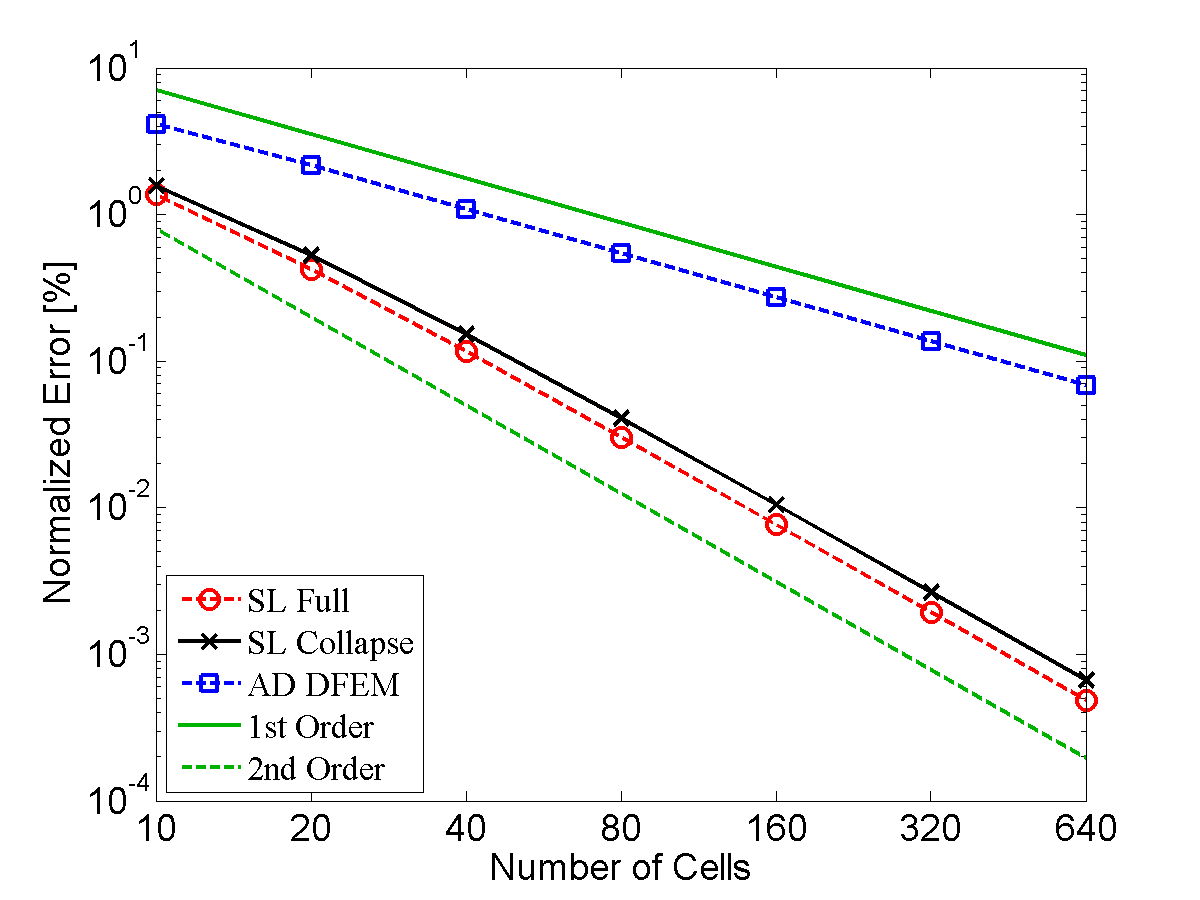
\includegraphics[width=9.5cm]{chapter5_depletion/FPA_P1_norm_err.png}
\caption{Normalized parasitic absorber fission product error for the depletion problem at end of cycle, for linear DFEM.}
\label{fig:depletion_NFPA_p1}
\end{figure}
%
\begin{figure}[!hbp]
\centering
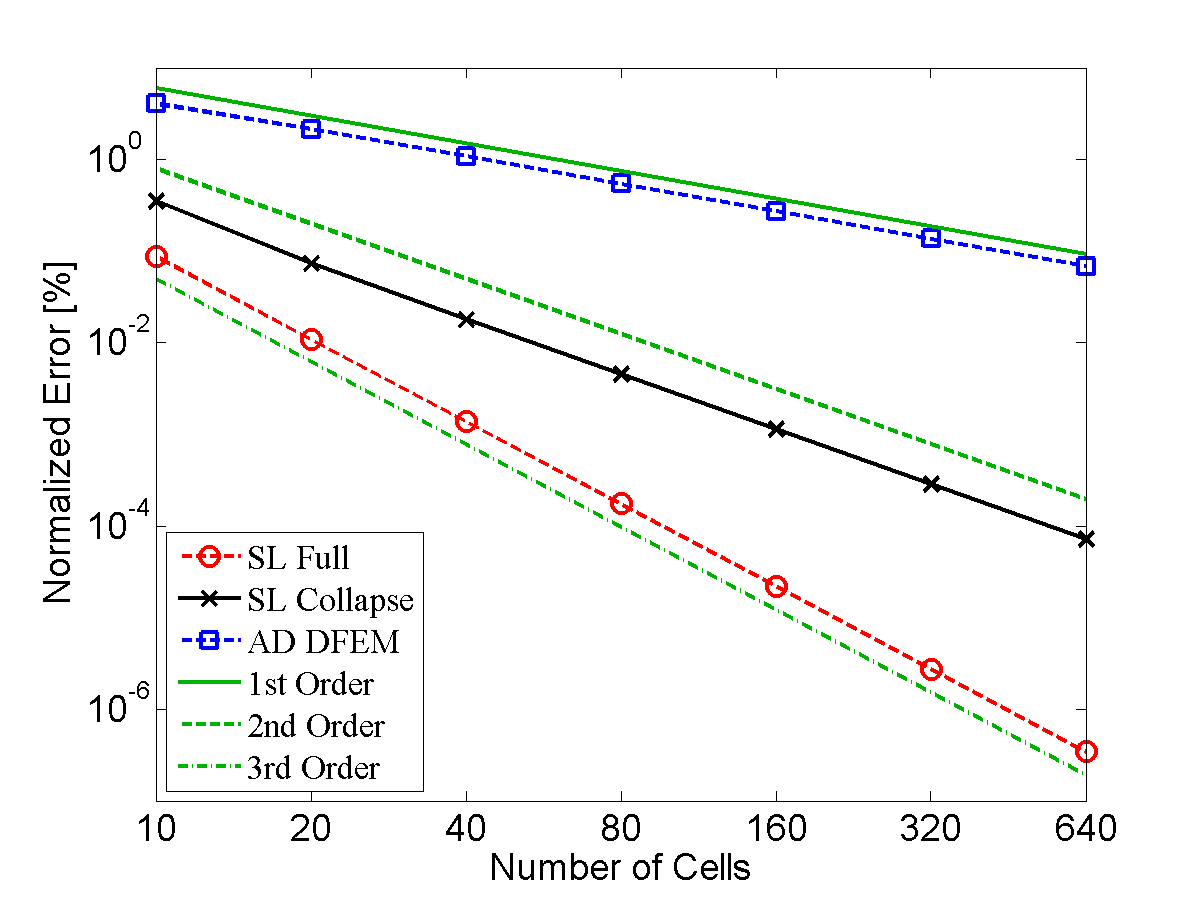
\includegraphics[width=9.5cm]{chapter5_depletion/FPA_P2_norm_err.png}
\caption{Normalized parasitic absorber fission product error for the depletion problem at end of cycle, for quadratic DFEM.}
\label{fig:depletion_NFPA_p2}
\end{figure}

\newpage

\begin{figure}[!htp]
\centering
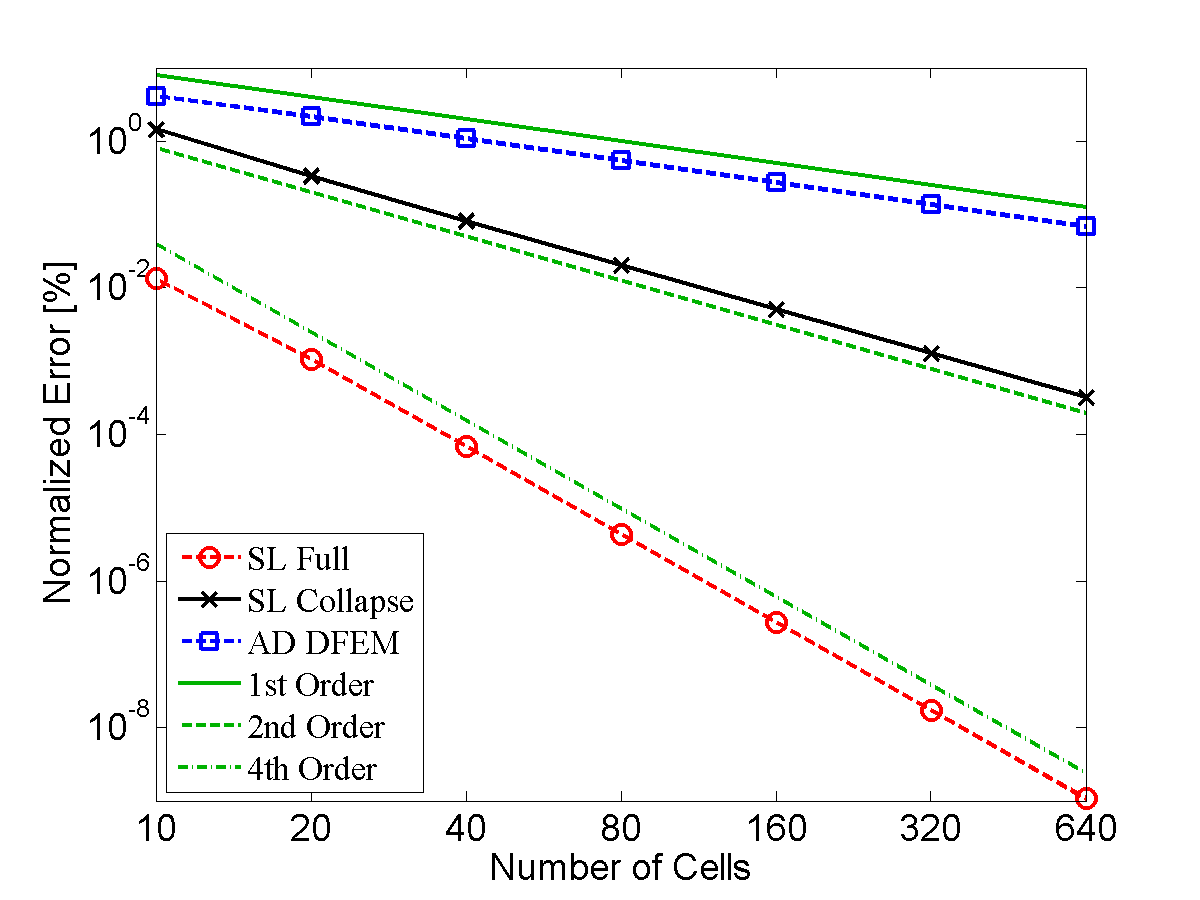
\includegraphics[width=9.5cm]{chapter5_depletion/FPA_P3_norm_err.png}
\caption{Normalized parasitic absorber fission product error for the depletion problem at end of cycle, for cubic DFEM.}
\label{fig:depletion_NFPA_p3}
\end{figure}
%
\begin{figure}[!hbp]
\centering
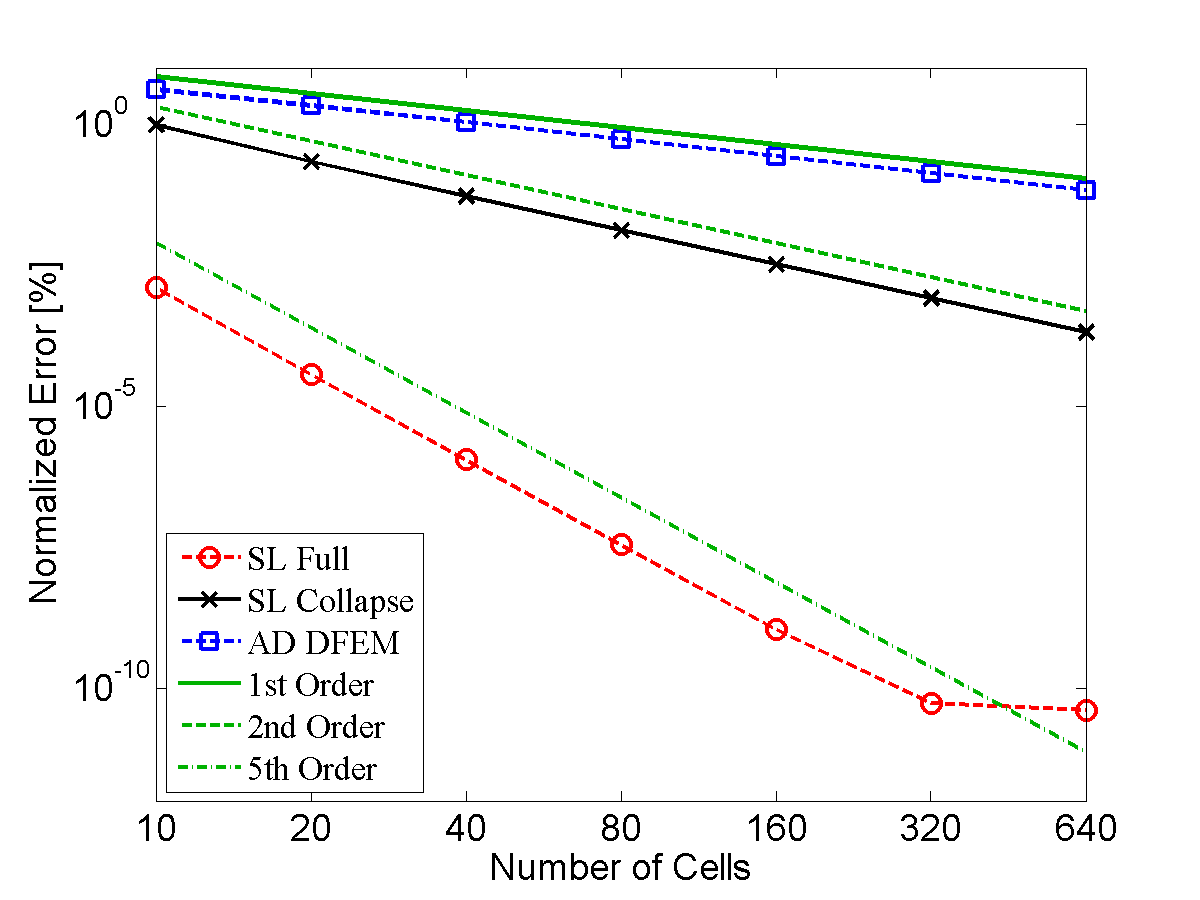
\includegraphics[width=9.5cm]{chapter5_depletion/FPA_P4_norm_err.png}
\caption{Normalized parasitic absorber fission product error for the depletion problem at end of cycle, for quartic DFEM.}
\label{fig:depletion_NFPA_p4}
\end{figure}  

\newpage

Examining the spatial convergence in nuclide densities, we make several observations.  
First, we note that the AD DFEM scheme (cell-wise average cross section, cell average nuclide density) achieves at most first-order convergence for all spatial nuclide density errors, regardless of the angular flux trial space degree.  
The AD DFEM scheme is limited to at most first-order convergence of the error in the spatial distribution of nuclides because the scalar flux is updated using only a cell-wise average cross section and only the cell average nuclide density is tracked.
Second, though the SL Collapse scheme expands nuclide density in a $P$ degree polynomial DFEM trial space, it achieves at most second-order $L^2$ convergence of the error in nuclides spatial distribution, for all trial  space polynomial degrees.  
SL Collapse is limited to at most second-order convergence of the spatial nuclide density solely because the scheme assumes a constant cross section in each cell when updating the scalar flux.  
The respective first-order and second-order convergence of the error in nuclide spatial distribution of the AD DFEM and SL Collapse scheme verifies the result observed in the pure absorber problem: assuming a cell-wise average cross section for coupled radiation transport problems limits the order of convergence of any quantity that depends on an interaction rate.
SL Full achieves $P+1$ order convergence of the error in spatial nuclide density for the fuel depletion problem, showing that coupled systems of equations involving radiation transport can be solved with arbitrary order of accuracy using high-order DFEM polynomial trial spaces and self-lumping numerical quadrature that explicitly accounts for the spatial variation of cross section within each cell.

